\documentclass{article}
\usepackage{mathpazo}
\usepackage{fullpage}
\usepackage{microtype}
\usepackage{amsmath}
\usepackage{graphicx}

\begin{document}
\section{Decomposable Learning/Training}

When I was doing a wall follow, I have noticed one interesting thing. To do a successful wall-follow you do not need to train the agent to wall-follow around the whole object. Let's consider the image below --- \\

\begin{figure}[h!]
\centering
	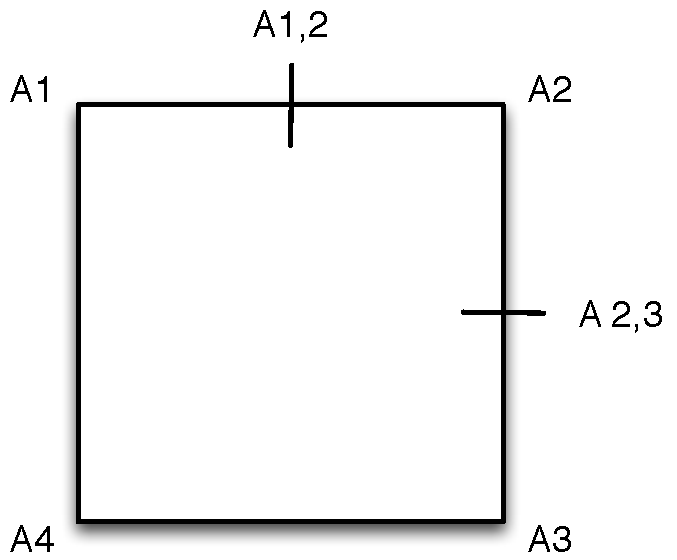
\includegraphics[width=0.33\textwidth]{wall-follow.pdf}
\end{figure}

Previously I was training the agent by starting from \(A_1\) to \(A_2\) and to \(A_3\); again from \(A_3\) to \(A_4\) and to \(A_1\), i.e. full clock-wise rotation. However, this learning process does not need to be a full rotation. If I train the agent to move around \(A_1\) to \(A_3\) the agent can successfully follow almost any simple geometrical object. Moreover, it can also do the wall-follow if we train the agent to move from just \(A_{1,2}\) to \(A_{2,3}\). Which suggests that the learning may not need to be exhaustive always. In this case, what the agent is doing is to utilize the ``perceptually aliased states'', since the corner \(A_1 - A_2 - A_3\) and \(A_3 - A_4 - A_1\) are ``perceptually aliased'' in terms of \emph{directio-to} and \emph{distance-from} the object. 

In other way, we can also say that the two features (i.e. \emph{direction-to} and \emph{distance-from}) are ``aliased-state-invariant'' when we are doing a ``wall-follow'' behavior.

So a I was wondering if a whole wall-follow could be made more general from training on a set of primitive objects like these --

\begin{figure}[h!]
\centering
	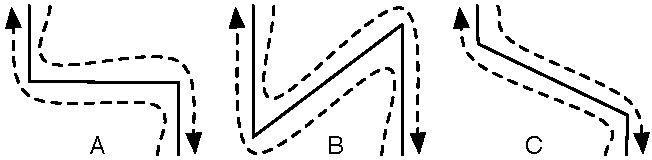
\includegraphics[width=0.80\textwidth]{walls.pdf}
\end{figure}


Here the object $A$ is has a turn of $90\,^{\circ}$, and the objects $B$ and $C$ has varying corner angles. Moreover, we will also train the agent for inside and outside corner. In this way we will train the agent with $N$ numbers of different primitive objects and test if it can do the wall-follow on complicated objects like the ``chinese character'' or around the ``vittorio'' objects in the HiTAB. 

A possible topic for investigation may be the minimum limit of decomposability of a large/complicated task, i.e. the minimum number of sub tasks that must be required to train the agent to achieve a very complicated maneuver, or what features are exactly need to be necessarily ``alised-state-invariant'' to successfully decompose a large complete maneuver to a set of independent small tasks -- so that we can only concentrate only on those to train the agent. 
\\

I am not sure if this problem is worth-pursuing or how to do the investigation/analysis if this seems really useful.
\end{document}
